% Author: Fevzi Yükseldi

\section{Entscheidungskern}

\subsection{Problemanalyse}
\subsubsection{Erweiterung des geometrischen Entscheidungskerns}
Da der Windfeld-Container\footnote{Ein Container, der viele verschiedene
Windfelder beinhaltet, auf die per Index zugegriffen werden kann.} für jede
Stunde jeweils ein Windfeld beinhaltet, müssen diese natürlich auch bei der
Berechnung berücksichtigt werden. Je nachdem zu welcher Zeit das Programm
ausgeführt wird, soll das dazugehörige Windfeld aus dem Container
herausgenommen und die Werte (die Windvektoren) davon benutzen werden. 

Wie auch schon erwähnt, wird für die Berechnung der Dauer die Windvektoren
benötigt. Deswegen kann es vorkommen, dass während der Fahrt von einem Knoten
zum Anderen die Windvektoren nicht mehr aktuell sind. Um dieses Problem aus
dem Weg zu räumen, soll nach jeder Berechnung die Dauer überprüft werden.
Falls die Dauer bis zu irgendeinem Knoten eine gewisse Grenze überschreitet,
soll das Windfeld gewechselt und dementsprechend  auch die neuen Windvektoren
benutzt werden. Diese Grenze befindet sich gerade in der Mitte der Zeitspanne
zwischen zwei aufeinander folgenden Windfelder. 

In unserem Fall beträgt diese Grenze 30, da wir für jede Stunde ein neues
Windfeld zur Verfügung haben. Somit wird bei jedem Knoten nach der Berechnung
überprüft, ob die Minutenzahl der Dauer bis zu diesem Knoten kleiner oder
grösser als diese Grenze ist. Falls sie kleiner ist, wird das aktuelle
Windfeld beibehalten und die Berechnung fortgesetzt. Falls sie aber grösser
ist, wird der Index des Windfelds um 1 erhöht und die Berechnung mit dem neuen
Wert wiederholt. D.h. Der Windvektor des Zielknotens wird erneuert, wobei der
Windvektor des Anfangsknotens gleich bleibt.

\subsubsection{Erstellung eines Entscheidungsbaums}
\label{aufg6:entscheidungsbaum}
Nach den Berechnungen soll mit den Werten ein Entscheidungsbaum erstellt
werden. Damit die Beziehungen zwischen den Knoten und die Dauer der Reisezeit
nicht verloren gehen bzw. nicht jedesmal erneut berechnet werden sollen,
werden alle nötigen Informationen in jedem Knoten abzuspeichern.
Dementsprechend soll dieser Entscheidungsbaum folgende Angaben beinhalten: 

\begin{itemize}
\item Vorheriger Knoten: Die Position des vorherigen Knotens in der Form \texttt{\{i,j\}}.
\item Aktueller Knoten: Die Position des aktuellen Knotens in der Form \texttt{\{i,j\}} .
\item Dauer: Die Dauer vom Anfangsknoten bis zu diesem Knoten.
\end{itemize}
Und sieht dann grafisch dargestellt wie folgt aus:
\begin{figure}[h!]
\centering
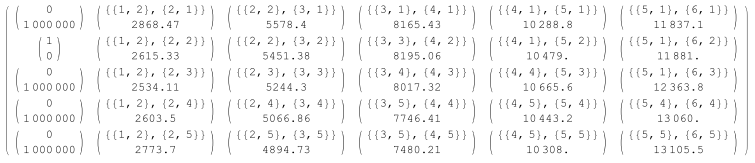
\includegraphics[width=1\linewidth]{img/grid_structure}
\caption{Struktur des Koordinatennetzes}
\label{gridnetConn}
\end{figure}

